\documentclass{standalone}
\usepackage[svgnames]{xcolor}
\usepackage{tikz}
\usetikzlibrary{matrix, positioning, arrows.meta, patterns}
\tikzset{>=Latex, Blue Box/.style={fill=RoyalBlue, text=white}, Red Box/.style={fill=FireBrick, text=white}, Data Property/.style={matrix of nodes, nodes={draw, minimum width=4ex, minimum height=4ex, anchor=center}, column sep=-0.4pt} }
\begin{document} 

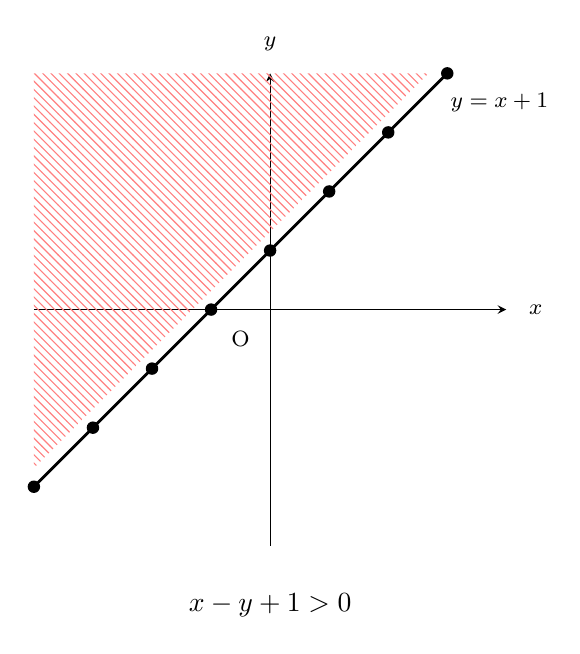
\begin{tikzpicture}[scale=0.75, >=stealth, baseline=-11pt]
\draw[->](-4,0) -- (4,0);\draw[->](0,-4) -- (0,4);
\draw(-0.5,-0.5) node {\footnotesize O};
\draw(4.5,0) node {\footnotesize $x$};
\draw(0,4.5) node {\footnotesize $y$};
\coordinate (A) at (-4,-3);
\coordinate (B) at (3,4);
	\draw[line width=1pt](A)--(B);
	\fill[pattern color=red!50, pattern=north west lines] ([yshift=9pt] A)--([xshift=-9pt] B)--(-4,4)--cycle;
	\draw(3,3.5) node[right,fill=white,inner sep=1pt]{\footnotesize \(y=x+1\)};
	\fill (-4,-3) circle (3pt)(-3,-2) circle (3pt)(-2,-1) circle (3pt)
    (-1,0) circle (3pt)(0,1) circle (3pt)(1,2) circle (3pt)(2,3) circle (3pt);
	\fill (3,4) circle (3pt);
	\draw(0,-5) node {$x-y+1>0$};
\end{tikzpicture}
\end{do}